% =============================================================================
% World Model Architectures in the Video Domain: A Systematic Literature Review
% Comparing Joint-Embedding Predictive Architectures (JEPA) and Generative Models
%
% IEEEtran conference format (A4). Compile with pdfLaTeX (Overleaf default).
% The bibliography is embedded below (no BibTeX run needed); references.bib is a
% companion file with the same entries.
% =============================================================================
\documentclass[conference,a4paper]{IEEEtran}

\usepackage{cite}
\usepackage{amsmath,amssymb,amsfonts}
\usepackage{graphicx}
\usepackage{xcolor}
\usepackage{booktabs}
\usepackage{array}
\usepackage{tabularx}
\newcolumntype{Y}{>{\raggedright\arraybackslash}X}
\usepackage{url}
\urlstyle{same}
\usepackage{tikz}
\usetikzlibrary{arrows.meta,positioning,calc}
\usepackage{balance}
\usepackage[hidelinks]{hyperref}

\newcounter{rqctr}
\newenvironment{rqlist}{%
  \begin{list}{\textbf{RQ\arabic{rqctr}}}{\usecounter{rqctr}%
    \setlength{\leftmargin}{2.5em}\setlength{\labelwidth}{2.2em}\setlength{\labelsep}{0.3em}%
    \setlength{\itemsep}{1pt}\setlength{\topsep}{2pt}\setlength{\parsep}{0pt}\setlength{\parskip}{0pt}}}%
  {\end{list}}

\begin{document}

\title{World Model Architectures in the Video Domain: A Systematic Literature Review Comparing Joint-Embedding Predictive Architectures (JEPA) and Generative Models}

\author{
\IEEEauthorblockN{1\textsuperscript{st} M. Hikari Reiziq Rakhmadinta}
\IEEEauthorblockA{\textit{Department of Information Technology} \\
\textit{Institut Teknologi Sepuluh Nopember}\\
Surabaya, Indonesia \\
5027241079@student.its.ac.id}
\and
\IEEEauthorblockN{2\textsuperscript{nd} Arya Bisma Putra Refman}
\IEEEauthorblockA{\textit{Department of Information Technology} \\
\textit{Institut Teknologi Sepuluh Nopember}\\
Surabaya, Indonesia \\
5027241036@student.its.ac.id}
\and
\IEEEauthorblockN{3\textsuperscript{rd} Ahmad Syauqi Reza}
\IEEEauthorblockA{\textit{Department of Information Technology} \\
\textit{Institut Teknologi Sepuluh Nopember}\\
Surabaya, Indonesia \\
50027241085@student.its.ac.id}
\and
\IEEEauthorblockN{4\textsuperscript{th} M. Fatihul Qolbi Ash Shidiqi}
\IEEEauthorblockA{\textit{Department of Information Technology} \\
\textit{Institut Teknologi Sepuluh Nopember}\\
Surabaya, Indonesia \\
5027241023@student.its.ac.id}
\and
\IEEEauthorblockN{5\textsuperscript{th} Rizka Wakhidatus Sholikah}
\IEEEauthorblockA{\textit{Department of Information Technology} \\
\textit{Institut Teknologi Sepuluh Nopember}\\
Surabaya, Indonesia \\
wakhidatus@its.ac.id \\
\textit{Corresponding author}}
}

\maketitle

\begin{abstract}
\textit{Background:} World models let intelligent systems predict how visual scenes evolve and are increasingly applied to video prediction, robot manipulation and autonomous driving. \textit{Problem:} Two architectural lineages compete: generative models that synthesise pixels, which are costly and prone to compounding error, and Joint-Embedding Predictive Architectures (JEPA), which predict abstract latent representations without pixel decoding. Evidence on their relative merits is scattered, and existing surveys offer taxonomies rather than protocol-driven syntheses of primary studies. \textit{Methodology:} We conducted a systematic literature review following Kitchenham and Charters and reported it with PRISMA 2020. Eight databases returned 2,812 records; after removing 115 duplicates, 2,697 records were screened against criteria that admit only peer-reviewed journal articles and exclude secondary studies and preprints. \textit{Key findings:} Fifteen primary studies published in 2024--2026 were retained and quality-assessed: eight JEPA or latent-predictive studies and seven generative (diffusion or flow-matching) studies. JEPA-lineage studies report gains in pre-training speed, probing error or latency against pixel-prediction, imitation-learning or language-model baselines, whereas generative studies report high-fidelity imagined rollouts at substantial computational cost, for example diffusion rollouts that dominate inference time. Direct comparisons between the two lineages within one study are scarce. \textit{Significance:} The review provides a transparent, reproducible evidence base and a five-question framework for comparing latent-prediction and generative world models in the video domain.
\end{abstract}

\begin{IEEEkeywords}
world models, joint-embedding predictive architecture, generative models, video prediction, diffusion models, systematic literature review, PRISMA
\end{IEEEkeywords}

%% ============================================================================
\section{Introduction}
%% ============================================================================

\subsection{World Models in the Video Domain}
A world model is a learned predictive model of how an environment evolves, which lets an agent anticipate the consequences of its actions without acting in the real world. Early recurrent world models showed that a compact learned model can serve as a simulator in which a policy is trained \cite{ha2018world}, and modern general-purpose agents learn such a model and improve their behaviour by imagining future scenarios \cite{hafner2025dreamerv3}; the principles of world-model learning and inference have also been reviewed from a theoretical perspective \cite{friston2021world}. When the observations are video, a world model must capture how scenes change under motion and action. Action-conditioned world models are useful for embodied agents only when their predicted futures remain controllable by actions and stable under long-horizon rollout \cite{wang2026sampopp}. They are now used for action-conditioned video prediction, visual planning and policy refinement in robot manipulation \cite{guo2026flowdreamer,jiang2026world4rl,qi2026gpc}; for simulating the evolution of 3D scenes, synthesising safety-critical scenarios and generating training data in autonomous driving \cite{wang2026occsora,guan2025accident,li2026nrseg}; and for visuomotor navigation of unmanned aerial vehicles \cite{zhao2024stc}. A further difficulty is that the capability of a pre-trained world model is typically restricted to its training distribution, which motivates online adaptation \cite{moon2026spread}.

\subsection{Two Competing Paradigms: Generative and Joint-Embedding Predictive}
World models for video differ most fundamentally in \emph{what they predict}. Generative world models synthesise future observations explicitly; recent examples use diffusion or flow-matching decoders to produce future frames or occupancy volumes \cite{jiang2026world4rl,guo2026flowdreamer,wang2026occsora,wang2026sampopp,guan2025accident}. High-fidelity imagined rollouts allow policies to be refined entirely inside a frozen world model \cite{jiang2026world4rl}, and synthetic scenes provide training data for perception and for safety-critical scenarios \cite{li2026nrseg,guan2025accident}. The same studies also expose the price of pixel-level generation: autoregressive prediction accumulates error over long horizons \cite{wang2026occsora}, generation noise can harm downstream learning \cite{li2026nrseg}, resolution and model capacity are limited by computational budgets \cite{jiang2026world4rl}, and diffusion rollouts can dominate inference time, requiring about 3~s per decision cycle in real-robot control \cite{qi2026gpc}.

Joint-Embedding Predictive Architectures (JEPA) take the opposite route. A predictor maps the representation of a context to the representation of a target, which an exponential-moving-average (EMA) encoder supplies under a stop-gradient, so no pixels are reconstructed \cite{bardes2024vjepa,assran2023ijepa}. Predicting in latent space allows the model to discard unpredictable or irrelevant detail \cite{bardes2024vjepa,vujinovic2026actjepa}. V-JEPA, trained only on video, reached 72.2\% on Something-Something-v2 with a frozen backbone and pre-trained roughly twice as fast as large pixel-prediction models \cite{bardes2024vjepa}. The idea has since been extended to imitation learning \cite{vujinovic2026actjepa}, object tracking \cite{chen2026gotjepa}, multimodal vehicular perception \cite{gupta2026lmjepa}, probabilistic patch matching \cite{gogos2026pijepa} and small-data regimes \cite{velez2026scott}. Its main limitation is that predictions are not images: visualising them requires a separately trained decoder \cite{bardes2024vjepa}. The two views therefore trade fidelity, interpretability, computational cost and robustness differently, and whether latent prediction can replace pixel generation for planning and control, or whether the two should be combined, remains open.

\subsection{Research Gap and Related Reviews}
Recent surveys map the growing world-model literature. Ding~\textit{et al.} organise world models into those that understand the present and those that predict the future \cite{ding2025survey}; Wang~\textit{et al.} review world models for robotic manipulation \cite{wang2026smartbot}; Kirchner~\textit{et al.} analyse design dimensions and uncertainty for physical AI \cite{kirchner2026survey}; and Chen and Liu cover connected automated driving \cite{chen2025cav}. Closest to our focus, Ahmad and Liu contrast generative (pixel-space) and latent (joint-embedding) world models by computational cost, surveying 15 representative models from 2023--2025 and noting that memory footprint is reported for only 40\% of them and power consumption for none \cite{ahmad2026cost}. These works are valuable overviews, but according to their abstracts they are taxonomic or design-space surveys; none describes a PRISMA-reported protocol with explicit eligibility criteria that restricts the evidence to peer-reviewed primary studies and compares JEPA-lineage and generative world models on downstream performance, evaluation practice and efficiency. Our own search retrieved 332 secondary studies, which we excluded by design because a systematic review synthesises primary evidence \cite{kitchenham2007guidelines}.

\subsection{Contributions and Outline}
This paper makes four contributions. First, it specifies and executes a reproducible protocol, with PICOC-based research questions, a search of eight databases using 68 database-specific queries, explicit eligibility criteria and a quality-assessment instrument, following Kitchenham and Charters \cite{kitchenham2007guidelines} and reporting according to PRISMA 2020 \cite{page2021prisma}. Second, it assembles a quality-assessed corpus of 15 peer-reviewed primary studies (Table~\ref{tab:studies}). Third, it characterises that corpus by architectural lineage, venue, domain and benchmark. Fourth, it formulates five research questions, on architectural paradigms, learning objectives, downstream performance and evaluation practice, efficiency trade-offs, and open challenges (Section~\ref{sec:rq}), that structure the comparison of JEPA and generative world models. The remainder of the paper is organised as follows. Section~\ref{sec:method} describes the review methodology, Section~III reports the results for RQ1--RQ5, Section~IV discusses the findings and threats to validity, and Section~V concludes.

%% ============================================================================
\section{Research Methodology}\label{sec:method}
%% ============================================================================

\subsection{Review Protocol and Guidelines}
The review follows the three phases of Kitchenham and Charters \cite{kitchenham2007guidelines}, namely planning, conducting and reporting, and is reported according to the PRISMA 2020 statement \cite{page2021prisma}. The protocol (PICOC, research questions, search strategy, eligibility criteria and quality-assessment instrument) is documented in a Kitchenham-style workbook maintained by the authors; the review was not registered in a public registry. % TODO(team): confirm "not registered"; add repository/data-availability link if the workbook is public.
Three refinements were made after the search and are reported here for transparency. First, to ensure that only peer-reviewed primary evidence was synthesised, exclusion criterion EC5 was operationalised as follows: conference papers, books, editorials and technical reports were removed through search filters, and secondary studies and preprints were excluded at screening. Secondary studies are excluded because a systematic review synthesises primary empirical evidence. Second, one report, a review article on world-model learning and inference \cite{friston2021world}, was excluded at the full-text stage under EC5. Third, inclusion criterion IC2 was applied inclusively to JEPA-lineage studies on images, because the Intervention explicitly includes image-based JEPA variants such as I-JEPA \cite{assran2023ijepa}.

\subsection{Defining the PICOC Framework}
The scope was defined with the PICOC framework (Table~\ref{tab:picoc}), which also guided the construction of the search strings.

\begin{table}[!t]
\caption{PICOC Formulation of the Review}
\label{tab:picoc}
\centering
\footnotesize
\renewcommand{\arraystretch}{1.1}
\begin{tabularx}{\columnwidth}{@{}l Y@{}}
\toprule
\textbf{Element} & \textbf{Operational definition} \\
\midrule
Population & AI systems that learn world models of an environment from visual or video observations (video prediction, robot manipulation, autonomous driving, UAV navigation). \\
Intervention & Joint-Embedding Predictive Architectures (JEPA family, e.g., I-JEPA, V-JEPA, ACT-JEPA) and related latent-predictive world models that predict in an abstract representation space without pixel decoding. \\
Comparison & Generative world models that predict or synthesise pixels or video (autoregressive, diffusion, flow-matching and reconstruction-based latent models). \\
Outcome & Downstream performance (video prediction: FVD, PSNR, SSIM, LPIPS; representation probing; planning and control: success rate, return), computational cost (FLOPs, memory, latency), sample and data efficiency, and representation stability (collapse, hallucination). \\
Context & Video-domain visual sequence modelling and interactive environments (video benchmarks, driving, robot manipulation, UAV navigation), in simulation and, where reported, on real systems; January 2018--September 2026. \\
\bottomrule
\end{tabularx}
\end{table}

\subsection{Research Questions}\label{sec:rq}
Five research questions were derived from the PICOC elements shown in parentheses:
\begin{rqlist}
\item Which architectural paradigms characterise JEPA-based and generative world models for video, and how did they evolve between 2018 and 2026? (P, I, C)
\item How do their learning objectives and representation spaces differ: latent feature prediction with EMA targets or regularisers versus pixel, diffusion or flow-matching objectives? (I, C, O)
\item How do the two lineages perform on downstream tasks (video or frame prediction, representation probing, planning and control), and which datasets, benchmarks and metrics are used to evaluate them? (I, C, O, Ctx)
\item What trade-offs in computational cost (FLOPs, memory, latency) and sample efficiency are reported? (I, C, O)
\item What open challenges and future directions are reported, including hybrid latent--generative designs? (I, C, Ctx)
\end{rqlist}

\subsection{Information Sources and Search Strategy}
Searches were executed on 22 September 2026 (IEEE Xplore on 23 September 2026) through the application programming interfaces of eight databases: CrossRef (1,067 records), OpenAlex (919), Springer Nature (232), ScienceDirect (214), Semantic Scholar (198), Scopus (86), IEEE Xplore (73) and PubMed (23), totalling 2,812 records. The search period was January 2018 to September 2026. No snowballing or hand-searching was performed, and Google Scholar was not used as a primary source. Search strings combined three concept blocks with AND, namely (1) world-model terms, (2) architecture terms (JEPA, joint embedding, generative, diffusion, latent dynamics) and (3) task and domain terms (video prediction, planning, model-based reinforcement learning, visual), with synonyms joined by OR. Each database received adapted queries, 68 in total (CrossRef 14, OpenAlex 10, Springer Nature 12, ScienceDirect 4, Semantic Scholar 10, Scopus 6, PubMed 5, IEEE Xplore 7), restricted by publication year and article type where the interface allowed. A representative Scopus query was TITLE-ABS-KEY((``world model'' \textsc{or} ``world models'') \textsc{and} (``video'' \textsc{or} ``visual'') \textsc{and} (``JEPA'' \textsc{or} ``generative'' \textsc{or} ``diffusion'' \textsc{or} ``autoregressive'')) with PUBYEAR $>$ 2017 and DOCTYPE(ar). The complete list of queries is recorded in the Search\_Strategy sheet of the workbook.

\subsection{Eligibility Criteria}
A record had to satisfy all inclusion criteria and no exclusion criterion. \textbf{Inclusion:} IC1, the article proposes, evaluates, analyses or compares a world-model architecture, including the JEPA/latent and generative/pixel lineages; IC2, the application domain involves video or sequential visual dynamics (frame prediction, spatio-temporal representations or visual planning); IC3, publication between January 2018 and September 2026; IC4, a peer-reviewed journal article with a clearly described method and empirical evaluation; IC5, full text accessible and written in English. \textbf{Exclusion:} EC1, duplicate record; EC2, outside the period; EC3, topic not relevant (not a world-model architecture, or unrelated to the JEPA-versus-generative contrast); EC4, non-visual domain (pure text or NLP); EC5, ineligible publication type, namely conference papers, books, editorials, technical reports, \emph{secondary studies} (surveys, reviews and systematic reviews) and \emph{non-peer-reviewed preprints} (arXiv or repository records without a journal version); EC6, full text unavailable. A record became a candidate only if all five inclusion criteria were marked ``Yes'' and no exclusion criterion was ``Yes''; this rule is computed by formula in the workbook.

\subsection{Study Selection Workflow and PRISMA 2020 Flow}
Fig.~\ref{fig:prisma} shows the flow of records. Of the 2,812 records, 115 duplicates (EC1), identified from normalised DOI and title, were removed, leaving 2,697 unique records for screening. The inclusion and exclusion flags of every record were stored in the Screening sheet of the workbook, where the Candidate/Exclude decision is computed by formula; flag assignment was script-assisted and rule-based, and no dedicated screening-automation software was used. % TODO(team): add number of reviewers, independence and disagreement handling if a manual double-screening was performed; none is documented in the repository.
In total 2,681 records were excluded: 2,196 under EC3 and 485 under EC5, of which 332 were secondary studies and 153 were non-peer-reviewed preprints; EC2, EC4 and EC6 were not triggered in the final run. The remaining 16 reports were sought and retrieved in full text, and all 16 were assessed for eligibility. One report, a review of world-model learning \cite{friston2021world}, was excluded as a secondary study (EC5), leaving 15 studies (15 reports) for quality assessment and synthesis.

\begin{figure*}[!t]
\centering
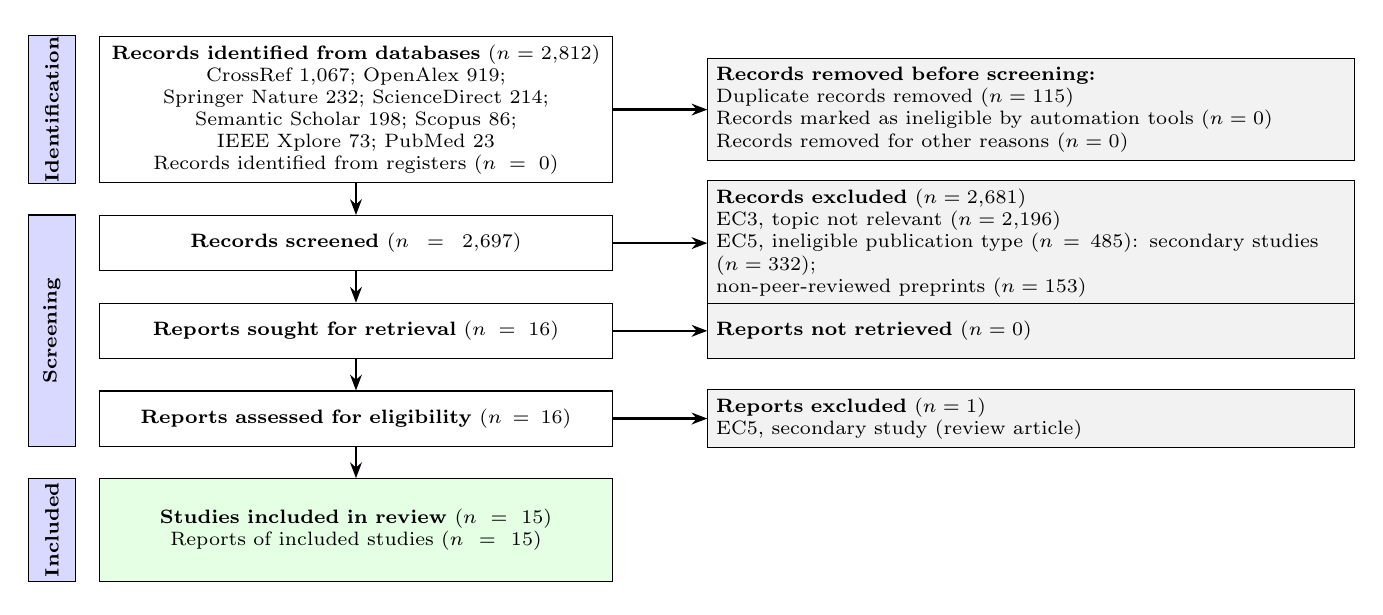
\begin{tikzpicture}[
  font=\scriptsize,
  node distance=4mm and 12mm,
  box/.style={draw, rectangle, align=center, inner sep=3pt, text width=6.3cm, minimum height=7mm, fill=white},
  ex/.style={draw, rectangle, align=left, inner sep=3pt, text width=8.0cm, minimum height=7mm, fill=gray!10},
  arr/.style={-{Stealth[length=2mm]}, thick}
]
\node[box] (ident) {\textbf{Records identified from databases} ($n=2{,}812$)\\
CrossRef 1,067; OpenAlex 919;\\
Springer Nature 232; ScienceDirect 214;\\
Semantic Scholar 198; Scopus 86;\\
IEEE Xplore 73; PubMed 23\\
Records identified from registers ($n=0$)};
\node[box, below=of ident] (screened) {\textbf{Records screened} ($n=2{,}697$)};
\node[box, below=of screened] (sought) {\textbf{Reports sought for retrieval} ($n=16$)};
\node[box, below=of sought] (assessed) {\textbf{Reports assessed for eligibility} ($n=16$)};
\node[box, below=of assessed, fill=green!10, minimum height=13mm] (included) {\textbf{Studies included in review} ($n=15$)\\
Reports of included studies ($n=15$)};

\node[ex, right=of ident] (dup) {\textbf{Records removed before screening:}\\
Duplicate records removed ($n=115$)\\
Records marked as ineligible by automation tools ($n=0$)\\
Records removed for other reasons ($n=0$)};
\node[ex, right=of screened] (excl) {\textbf{Records excluded} ($n=2{,}681$)\\
EC3, topic not relevant ($n=2{,}196$)\\
EC5, ineligible publication type ($n=485$): secondary studies ($n=332$);\\
non-peer-reviewed preprints ($n=153$)};
\node[ex, right=of sought] (notret) {\textbf{Reports not retrieved} ($n=0$)};
\node[ex, right=of assessed] (excl2) {\textbf{Reports excluded} ($n=1$)\\
EC5, secondary study (review article)};

\draw[arr] (ident) -- (screened);
\draw[arr] (screened) -- (sought);
\draw[arr] (sought) -- (assessed);
\draw[arr] (assessed) -- (included);
\draw[arr] (ident) -- (dup);
\draw[arr] (screened) -- (excl);
\draw[arr] (sought) -- (notret);
\draw[arr] (assessed) -- (excl2);

\draw[fill=blue!15] ($(ident.north west)+(-9mm,0)$) rectangle ($(ident.south west)+(-3mm,0)$)
  node[pos=.5, rotate=90, font=\scriptsize\bfseries] {Identification};
\draw[fill=blue!15] ($(screened.north west)+(-9mm,0)$) rectangle ($(assessed.south west)+(-3mm,0)$)
  node[pos=.5, rotate=90, font=\scriptsize\bfseries] {Screening};
\draw[fill=blue!15] ($(included.north west)+(-9mm,0)$) rectangle ($(included.south west)+(-3mm,0)$)
  node[pos=.5, rotate=90, font=\scriptsize\bfseries] {Included};
\end{tikzpicture}
\caption{PRISMA 2020 flow diagram of identification, screening and inclusion (databases only; searches executed 22--23 September 2026). EC = exclusion criterion.}
\label{fig:prisma}
\end{figure*}

\subsection{Quality Assessment Instrument}
Each candidate report was scored on eight criteria derived from the review protocol: QA1, clarity of aims and research questions; QA2, transparent description of the world-model architecture, including loss function, latent representation and input--output flow; QA3, reproducibility of the experimental setup (datasets, training procedure and baselines); QA4, relevance of the evaluation metrics to world modelling (e.g., FVD, PSNR/SSIM, probing accuracy, success rate); QA5, empirical comparison against relevant baselines within or across the two lineages; QA6, objective and quantitative reporting of results; QA7, honest discussion of limitations, failure modes, hallucination or collapse; and QA8, consistency of the conclusions with the results and contribution to the JEPA-versus-generative debate. Each criterion was scored 1 (low), 2 (moderate) or 3 (high), so the total ranges from 8 to 24 and the percentage is the total divided by 24. Studies scoring at least 75\% were classified as Final, 60--74.9\% as Review and below 60\% as Exclude. All 15 retained studies were rated Final (22--24 of 24; mean 23.7), as listed in Table~\ref{tab:studies}.

\subsection{Data Extraction and Qualitative Synthesis}
Data were extracted with an 18-attribute form: identifier, title, authors, year, venue, DOI, URL, research aim, research question, methodology, dataset or sample, technology or approach (JEPA, generative or comparative), evaluation metrics, key findings, limitations, future work, relevant research question and extraction notes. Bibliographic attributes were verified against publisher records (CrossRef and the TMLR record) and technical attributes against the study report itself, and any extracted value that disagreed with its source was corrected. % TODO(team): FP-04, FP-06, FP-08 and FP-10 were verified from abstracts only; re-verify against full texts and finalise the corresponding rows of Table II.
Because the studies differ in domain, benchmark and metric, the synthesis is qualitative and thematic rather than a meta-analysis: studies are grouped by architectural lineage (JEPA or latent-predictive versus generative) and compared along the dimensions of RQ1--RQ5, with each research question answered in its own subsection. Threats to validity addressed by design are publication bias from excluding preprints and conference papers, coverage bias from restricting the search to journal articles indexed in eight databases, and interpretation bias from overlapping lineage categories, which is limited by classifying each study according to its dominant contribution. Table~\ref{tab:studies} summarises the corpus. Studies marked \textsuperscript{\dag} do not describe their model as a world model and are included as JEPA-lineage evidence under the PICOC Intervention; this and the inclusion of two image-only studies are limitations of the corpus.

\begin{table*}[!t]
\caption{Characteristics of the 15 Included Primary Studies}
\label{tab:studies}
\centering
\scriptsize
\setlength{\tabcolsep}{2.5pt}
\renewcommand{\arraystretch}{1.1}
\begin{tabularx}{\textwidth}{@{}l l c l l Y Y c@{}}
\toprule
\textbf{ID} & \textbf{Study} & \textbf{Year} & \textbf{Venue} & \textbf{Category} & \textbf{Method / backbone} & \textbf{Domain and benchmarks} & \textbf{QA} \\
\midrule
FP-01 & Bardes et al.~\cite{bardes2024vjepa} & 2024 & TMLR & JEPA\textsuperscript{\dag} & V-JEPA: masked feature prediction with $\ell_1$ loss to an EMA target; ViT-L/H encoder & Video: pre-trained on VideoMix2M (2M videos); K400, SSv2, AVA, ImageNet-1K (frozen probing) & 24 \\
FP-02 & Vujinovi{\'c} \& Kova{\v{c}}evi{\'c}~\cite{vujinovic2026actjepa} & 2026 & IEEE Access & JEPA & ACT-JEPA: imitation learning plus latent JEPA; predicts action chunks and latent observations & Simulated manipulation from images: Push-T, Meta-World, ManiSkill & 23 \\
FP-03 & Chen et al.~\cite{chen2026gotjepa} & 2026 & IEEE TCSVT & JEPA\textsuperscript{\dag} & GOT-JEPA: teacher--student prediction of tracking models; OccuSolver; DINOv2 ViT-L & Video object tracking: AVisT, NfS, OTB-100, GOT-10k, LaSOT, TrackingNet, VOT2022 & 24 \\
FP-04 & Gogos et al.~\cite{gogos2026pijepa} & 2026 & Pattern Recognit. Lett. & JEPA\textsuperscript{\dag} (image) & Probabilistic I-JEPA: matching distributions of masked-patch representations & Image classification and transfer learning (images only) & 22 \\
FP-05 & Gupta \& Sultana~\cite{gupta2026lmjepa} & 2026 & Sensors & JEPA\textsuperscript{\dag} & LM-JEPA: multimodal latent JEPA with lightweight VLM and selective latent transmission & Driving perception and QA: BDD100K, nuScenes-QA; CARLA closed loop & 23 \\
FP-06 & Zhao et al.~\cite{zhao2024stc} & 2024 & IEEE TAI & Latent-predictive (contrastive) & STC: RNN dynamics model with multi-objective contrastive loss; pre-trained encoder & UAV visual navigation: simulated environment and out-of-domain data & 24 \\
FP-07 & V{\'e}lez-Garc{\'\i}a et al.~\cite{velez2026scott} & 2026 & CVIU & JEPA\textsuperscript{\dag} (image) & SCOTT sparse convolutional tokenizer with MIM-JEPA (EMA target) & Images: Flowers-102, Pets-37, ImageNet-100 & 23 \\
FP-08 & Moon \& Kim~\cite{moon2026spread} & 2026 & IEEE RA-L & Latent world model & SPREAD: frozen pre-trained world model with LoRA adapters for online adaptation & Robot control under visual and dynamics shifts & 24 \\
FP-09 & Jiang et al.~\cite{jiang2026world4rl} & 2026 & IEEE RA-L & Generative (diffusion) & World4RL: EDM-style diffusion world model; two-hot actions; policy refinement in imagination & Meta-World (6 tasks); real Franka Panda (6 tasks) & 24 \\
FP-10 & Wang et al.~\cite{wang2026sampopp} & 2026 & IEEE TPAMI & Generative (flow matching) & SAMPO++: temporal autoregression with scale-wise flow matching in a latent pyramid & Manipulation, visual planning, model-based RL; driving video prediction & 24 \\
FP-11 & Wang et al.~\cite{wang2026occsora} & 2026 & IEEE TIP & Generative (diffusion) & OccSora: 4D occupancy tokenizer with trajectory-conditioned diffusion transformer & Driving: nuScenes with Occ3D annotations & 24 \\
FP-12 & Li et al.~\cite{li2026nrseg} & 2026 & IEEE TIP & Generative\textsuperscript{\ddag} (data) & NRSeg: noise-resilient learning from synthetic data of driving world models (PGCM, BiDPP, HLSE) & BEV segmentation: nuScenes (domain adaptation, semi-supervised) & 24 \\
FP-13 & Guo et al.~\cite{guo2026flowdreamer} & 2026 & IEEE RA-L & Generative (diffusion) & FlowDreamer: U-Net 3D scene flow with fine-tuned Stable Diffusion renderer & Manipulation: SimplerEnv RT-1, Language Table, VP2 (RoboDesk, Robosuite) & 24 \\
FP-14 & Guan et al.~\cite{guan2025accident} & 2025 & Commun. Eng. & Generative (diffusion) & Stable-Diffusion-based driving world model for scene generation; dynamic GCN anticipation & Accident anticipation: DAD, A3D, CCD, new AoTA & 24 \\
FP-15 & Qi et al.~\cite{qi2026gpc} & 2026 & IEEE RA-L & Generative (diffusion) & GPC: frozen diffusion policy with image-space diffusion world model (rank and optimise) & Manipulation: Push-T, block stacking and others; real robot & 24 \\
\bottomrule
\end{tabularx}
\\[2pt]
\begin{minipage}{\textwidth}
\footnotesize
\textsuperscript{\dag}~Does not describe itself as a world model; included as JEPA-lineage evidence under the PICOC Intervention.\quad
\textsuperscript{\ddag}~Uses synthetic data from generative driving world models rather than proposing one.\quad
Years and venues follow the publisher record. QA is the total recorded in the review workbook (scale 1--3 per criterion; maximum 24).
\end{minipage}
\end{table*}

% ---------------------------------------------------------------------------
% TODO (subsequent sections; outside the scope of this version of the file)
% \section{Results}                 % III-A study characteristics; III-B ... III-F: one subsection per RQ1--RQ5
% \section{Discussion}              % IV: interpretation, comparison with prior surveys, threats to validity
% \section{Conclusion and Future Work}
% ---------------------------------------------------------------------------

\balance

% BEGIN-BIB (generated; entries ordered by first citation)
\begin{thebibliography}{00}
\bibitem{ha2018world}
D. Ha and J. Schmidhuber, ``Recurrent world models facilitate policy evolution,'' in \emph{Proc. Adv. Neural Inf. Process. Syst. (NeurIPS)}, vol.~31, 2018. [Online]. Available: \url{https://papers.nips.cc/paper_files/paper/2018/hash/2de5d16682c3c35007e4e92982f1a2ba-Abstract.html}

\bibitem{hafner2025dreamerv3}
D. Hafner, J. Pasukonis, J. Ba, and T. Lillicrap, ``Mastering diverse control tasks through world models,'' \emph{Nature}, vol.~640, no.~8059, pp.~647--653, Apr. 2025, doi: \url{10.1038/s41586-025-08744-2}.

\bibitem{friston2021world}
K. Friston, R. J. Moran, Y. Nagai, T. Taniguchi, H. Gomi, and J. Tenenbaum, ``World model learning and inference,'' \emph{Neural Netw.}, vol.~144, pp.~573--590, Dec. 2021, doi: \url{10.1016/j.neunet.2021.09.011}.

\bibitem{wang2026sampopp}
S. Wang, S. Zhou, H. Dong, K. Xia, G. Hua, and L. Wang, ``Action-controlled scale-wise flow matching for embodied world models,'' \emph{IEEE Trans. Pattern Anal. Mach. Intell.}, early access, 2026, doi: \url{10.1109/TPAMI.2026.3727986}.

\bibitem{guo2026flowdreamer}
J. Guo, X. Ma, Y. Wang, M. Yang, H. Liu, and Q. Li, ``FlowDreamer: A RGB-D world model with flow-based motion representations for robot manipulation,'' \emph{IEEE Robot. Autom. Lett.}, vol.~11, no.~3, pp.~2466--2473, Mar. 2026, doi: \url{10.1109/LRA.2026.3653273}.

\bibitem{jiang2026world4rl}
Z. Jiang \emph{et al.}, ``World4RL: Diffusion world models for policy refinement with reinforcement learning for robotic manipulation,'' \emph{IEEE Robot. Autom. Lett.}, vol.~11, no.~10, pp.~12240--12247, Oct. 2026, doi: \url{10.1109/LRA.2026.3728345}.

\bibitem{qi2026gpc}
H. Qi, H. Yin, A. Zhu, Y. Du, and H. Yang, ``Inference-time enhancement of generative robot policies via predictive world modeling,'' \emph{IEEE Robot. Autom. Lett.}, vol.~11, no.~5, pp.~5534--5541, May 2026, doi: \url{10.1109/LRA.2026.3673995}.

\bibitem{wang2026occsora}
L. Wang \emph{et al.}, ``OccSora: 4D occupancy generation models as world simulators for autonomous driving,'' \emph{IEEE Trans. Image Process.}, vol.~35, pp.~4947--4960, 2026, doi: \url{10.1109/TIP.2026.3687468}.

\bibitem{guan2025accident}
Y. Guan, H. Liao, C. Wang, X. Liu, J. Zhang, and Z. Li, ``World model-based end-to-end scene generation for accident anticipation in autonomous driving,'' \emph{Commun. Eng.}, vol.~4, no.~1, Art.~no.~144, Aug. 2025, doi: \url{10.1038/s44172-025-00474-7}.

\bibitem{li2026nrseg}
S. Li, F. Teng, Y. Cao, K. Yang, Z. Li, and Y. Wang, ``NRSeg: Noise-resilient learning for BEV semantic segmentation via driving world models,'' \emph{IEEE Trans. Image Process.}, vol.~35, pp.~3038--3052, 2026, doi: \url{10.1109/TIP.2026.3671686}.

\bibitem{zhao2024stc}
J. Zhao, Y. Wang, Z. Cai, N. Liu, K. Wu, and Y. Wang, ``Learning visual representation for autonomous drone navigation via a contrastive world model,'' \emph{IEEE Trans. Artif. Intell.}, vol.~5, no.~3, pp.~1263--1276, Mar. 2024, doi: \url{10.1109/TAI.2023.3283488}.

\bibitem{moon2026spread}
J. Moon and S.-W. Kim, ``SPREAD: Scalable pre-trained world model for adaptive dynamics model,'' \emph{IEEE Robot. Autom. Lett.}, vol.~11, no.~6, pp.~7460--7467, Jun. 2026, doi: \url{10.1109/LRA.2026.3688061}.

\bibitem{bardes2024vjepa}
A. Bardes \emph{et al.}, ``Revisiting feature prediction for learning visual representations from video,'' \emph{Trans. Mach. Learn. Res.}, Aug. 2024. [Online]. Available: \url{https://openreview.net/forum?id=QaCCuDfBk2}

\bibitem{assran2023ijepa}
M. Assran \emph{et al.}, ``Self-supervised learning from images with a joint-embedding predictive architecture,'' in \emph{Proc. IEEE/CVF Conf. Comput. Vis. Pattern Recognit. (CVPR)}, Jun. 2023, pp.~15619--15629, doi: \url{10.1109/CVPR52729.2023.01499}.

\bibitem{vujinovic2026actjepa}
A. Vujinovi{\'c} and A. Kova{\v{c}}evi{\'c}, ``ACT-JEPA: Novel joint-embedding predictive architecture for efficient policy representation learning,'' \emph{IEEE Access}, vol.~14, pp.~78895--78906, 2026, doi: \url{10.1109/ACCESS.2026.3696039}.

\bibitem{chen2026gotjepa}
S.-F. Chen, J.-C. Chen, I.-H. Jhuo, and Y.-Y. Lin, ``GOT-JEPA: Generic object tracking with model adaptation and occlusion handling using joint-embedding predictive architecture,'' \emph{IEEE Trans. Circuits Syst. Video Technol.}, vol.~36, no.~7, pp.~10836--10851, Jul. 2026, doi: \url{10.1109/TCSVT.2026.3675005}.

\bibitem{gupta2026lmjepa}
A. Gupta and A. Sultana, ``Object detection and scene perception for connected and autonomous vehicles using LM-JEPA,'' \emph{Sensors}, vol.~26, no.~15, Art.~no.~4894, Aug. 2026, doi: \url{10.3390/s26154894}.

\bibitem{gogos2026pijepa}
L. Gogos, D. Katsikas, N. Passalis, and A. Tefas, ``Probabilistic image-based joint embedding predictive architecture,'' \emph{Pattern Recognit. Lett.}, vol.~207, pp.~234--240, Sep. 2026, doi: \url{10.1016/j.patrec.2026.07.005}.

\bibitem{velez2026scott}
C. V{\'e}lez-Garc{\'\i}a, M. Cazorla, and J. Pomares, ``Escaping the big data paradigm in self-supervised representation learning,'' \emph{Comput. Vis. Image Underst.}, vol.~266, Art.~no.~104698, Mar. 2026, doi: \url{10.1016/j.cviu.2026.104698}.

\bibitem{ding2025survey}
J. Ding \emph{et al.}, ``Understanding world or predicting future? A comprehensive survey of world models,'' \emph{ACM Comput. Surv.}, vol.~58, no.~3, pp.~1--38, 2025, doi: \url{10.1145/3746449}.

\bibitem{wang2026smartbot}
F. Wang \emph{et al.}, ``World models for robotic manipulation: A survey,'' \emph{SmartBot}, Art.~no.~e70053, Aug. 2026, doi: \url{10.1002/smb2.70053}.

\bibitem{kirchner2026survey}
S. Kirchner, N. Purschke, and A. Knoll, ``A survey of world models for physical AI with uncertainty representation and control,'' \emph{Discov. Artif. Intell.}, vol.~6, no.~1, Art.~no.~1037, Sep. 2026, doi: \url{10.1007/s44163-026-02122-1}.

\bibitem{chen2025cav}
N. Chen and X. Liu, ``Research on world models for connected automated driving: Advances, challenges, and outlook,'' \emph{Appl. Sci.}, vol.~15, no.~16, Art.~no.~8986, Aug. 2025, doi: \url{10.3390/app15168986}.

\bibitem{ahmad2026cost}
H. Ahmad and H. Liu, ``The cost of dreaming: A survey of computational constraints in generative and latent world models,'' \emph{IEEE Comput. Intell. Mag.}, early access, 2026, doi: \url{10.1109/MCI.2026.3713292}.

\bibitem{kitchenham2007guidelines}
B. Kitchenham and S. Charters, ``Guidelines for performing systematic literature reviews in software engineering,'' Keele Univ. and Univ. Durham, U.K., EBSE Tech. Rep. EBSE-2007-01, 2007.

\bibitem{page2021prisma}
M. J. Page \emph{et al.}, ``The PRISMA 2020 statement: An updated guideline for reporting systematic reviews,'' \emph{BMJ}, vol.~372, Art.~no.~n71, Mar. 2021, doi: \url{10.1136/bmj.n71}.
\end{thebibliography}
% END-BIB

\end{document}
